\documentclass[../Ansoegning.tex]{subfiles}
\begin{document}
\begin{center}
    \Large{\textbf{Karakterudskrift for nuværende videregående uddannelse}}\vspace{-0.7cm}
\end{center}
Herunder fremgår mit nuværende karakterblad, indeholdende samtlige kurser og karakterene af disse til og med min fjerde semester. Jeg har på nuværende tidspunkt et vægtet gennemsnit på \avgKar:
\begin{minipage}{1\textwidth}
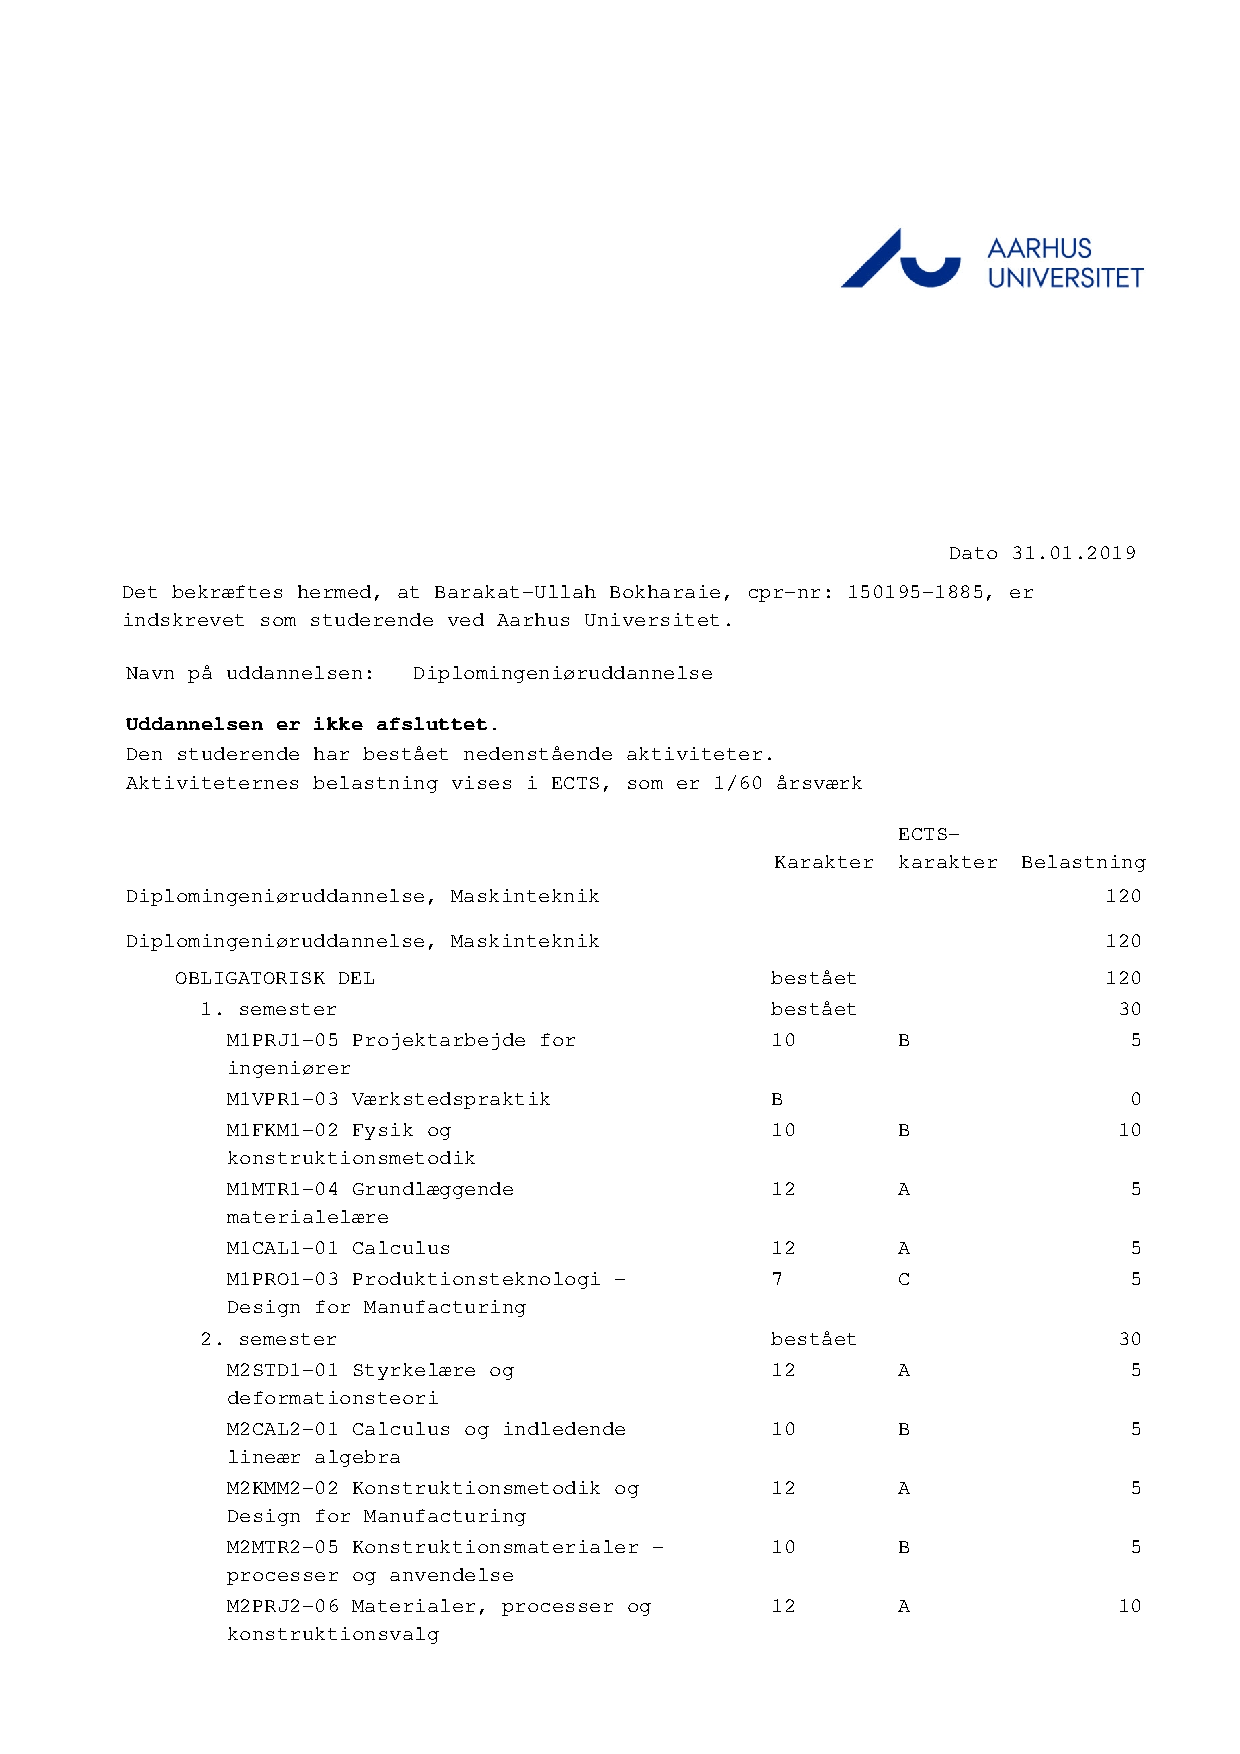
\includepdf[pages={1}, scale=0.85, pagecommand={\label{sec:flaskehaeldning}}, offset=0 -0.1cm]{Eksterne_filer/karakterudskrift.pdf}
\end{minipage}
    \newpage
\begin{minipage}{1\textwidth}
\includepdf[pages={2}, scale=0.85, pagecommand={\label{sec:flaskehaeldning}}, offset=0 -1cm]{Eksterne_filer/karakterudskrift.pdf}
\end{minipage}
\end{document}